\documentclass{beamer}
\usepackage{tikz}

\usepackage{graphicx}
% Required package
\usepackage{subcaption}
% ---
% Configurações de aparência do PDF final


\usepackage{xcolor}

\usepackage{mathtools}

\usepackage[portuguese]{babel}
\usepackage[brazilian,hyperpageref]{backref}	 % Paginas com as citações na bibl
\usepackage[alf]{abntex2cite}	% Citações padrão ABNT

%Information to be included in the title page:
\title{Implementação de um modelo de classificação de áreas irregulares na Floresta Amazônica baseado em Transformers Visuais}


\author{Victor Moraes}
\institute{UFMG}
\date{2022}


\begin{document}

\frame{\titlepage}

\begin{frame}
\frametitle{Motivação}  

    \begin{figure}[!h]
    \centering
    \includegraphics[width=0.6\columnwidth]{../Imagens/Ti-Munduruku-Foto_Marizilda_Cruppe_Amazônia_Real.jpg}
    \caption[width=0.2\columnwidth]{\\\small Garimpo ilegal na Terra Indígena Munduruku, município de Jacareacanga. Foto: Marizilda Cruppe/Amazônia Real}
    \label{fig:garimpo}
    \end{figure}

    % A Floresta Amazônica enfrenta um acumulo histórico de degradação, além de crescentes níveis de desmatamento e destruição de habidats, seja por agricultura, mineração, extração e pecuária ilegais. Para diagnisticar tais degradações sobre a imensa área que a floresta cobre, o instuturo nacional de pesquisas espaciais possui satélites que realizam o sensoriamento remoto da região, para diagnisticar utilizando vários espectros e áreas abrangentes. Contudo até então foram usados satélites de baixa resolução para o espectro visível. Recentemente O INPE conta com satélites do espectro visiível de altissimas resoluções e que combinados com técnicas de visão computacional e aprendizado profundo, podem diagnisticar com presição degradações esparças e de pequena escalas, ou mesmo ocultas.

\end{frame}


\begin{frame}
    \frametitle{Revisão bibliográfica }
\begin{itemize}
    \item Domínio do problema: Sensoriamento remoto
    \item Aprendizado de máquina
    \item Redes convolucionais
    \item Transformers
    \item Trabalhos anteriores
\end{itemize}

    % Neste capítulo, será apresentado inicialmente definições do domínio do problema de classificação e identificação de cenas em sensoriamento remoto na seção~\ref{sec:Cap2_dominio}, bem como suas características e contexto. Seguindo por um apanhado teórico da seção envolvendo aprendizado de máquina, redes neurais, redes neurais profundas, convolucionais e~\textit{transformers}, no que tange interseções com possíveis soluções para o problema. E por fim, na seção~\ref{sec:Cap2_revisao_literatura} uma revisão da literatura e do atual estado da arte no que tange o problema de classificação visual no que tange a sensoriamento remoto. Apresentando trabalhos que envolveram soluções tanto para o campo, quanto para implementações de redes neurais profundas.
\end{frame}


\begin{frame}
    \frametitle{Revisão bibliográfica - Sensoriamento remoto}
    \begin{figure}[!ht]
        \centering
        \includegraphics[width=0.9\columnwidth]{
            ../Imagens/instrutorgis\_sensoriamento\_remoto\_ilustracao.png
        }
        \caption{Sensoriamento remoto Foto:\cite{InstrutorGIS}}
    \label{fig:sensoriamento}
    \end{figure}
    % O problema em questão, de identificação de regiões com garimpo em imagens de satélite, e pertencem ao campo de sensoriamento remoto. O sensoriamento remoto consiste em aquistar ou analisar medições de uma região geográfica terrestre, ou atmosférica. Podem ser realizadas por imagens aéreas ou por satélites, podendo abranger diferentes partes do espectro eletromagnético.Frequentemente consistem em métodos de aquisição ou processamento de sinais e imagens, para obter características ou reconhecer padrões em tais localidades~\cite{emery2017introduction}.O termo foi cunhado referir-se a medição realizada por algum meio indireto ou “remoto”, em vez de um contato direto com sensores no ambiente medido~\cite{emery2017introduction}.
    \end{frame}

\begin{frame}
\frametitle{Revisão bibliográfica - Aprendizado de máquina}
Definição:
“Campo de estudos que visa a dar computadores a habilidade de aprender sem serem explicitamente programados para determinada tarefa." ~\cite{Samuel1959SomeSI}

“Um algoritmo dito conseguir uma experiência E com respeito a determinada classe de tarefas T e com medidas de desempenho P, se seu desempenho nas tarefas em T, medidas por P, melhoram a partir da experiência E.” ~\cite{Mitchell97} 

% Aprendizado de máquina é um campo que estuda algorítimos capazes de aprender e realizar inferências a partir de dados. O termo foi cunhado em ~\cite{Samuel1959SomeSI}, como “Campo de estudos que visa a dar computadores a habilidade de aprender sem serem explicitamente programados para determinada tarefa.”.

%Já em~\cite{Mitchell97} define um algorítimo de aprendizado como “Um algoritmo dito conseguir uma experiência E com respeito a determinada classe de tarefas T e com medidas de desempenho P, se seu desempenho nas tarefas em T, medidas por P, melhoram a partir da experiência E.”

%Para melhor entender cada constituinte dessa definição, podemos utilizar de um exemplo. A tarefa T temos como exemplo o problema de classificação, que consiste do algorítimo responder quais das k categorias para o qual ele experimentou em E, certas amostras de entradas pertencem. Para resolver tal tarefa, tal algorítimo de aprendizado deve produzir uma função \(f:\Re^n\rightarrow \{1,\ldots,k\}\). Quando \( y=f(x) \), o modelo atribui uma entrada descrita pelo por \(x\), que nosso caso constitui uma amostra de entrada, a uma categoria identificada por um código numérico \(y\). Uma variante do mesmo problema é em vez de classificar qual classe, retornar a distribuição de probabilidade sobre as classes~\cite{GoodBengCour16}. A medida de desempenho P, necessária para avaliar as habilidades de um dado algorítimo. Tal medida de desempenho é geralmente atrelada ao tipo de tarefa sendo realizada pelo sistema. 
\end{frame}


\begin{frame}
    \frametitle{Revisão bibliográfica - Aprendizado de máquina}
    Definição:
    “Campo de estudos que visa a dar computadores a habilidade de aprender sem serem explicitamente programados para determinada tarefa." ~\cite{Samuel1959SomeSI}
    
    “Um algoritmo dito conseguir uma experiência E com respeito a determinada classe de tarefas T e com medidas de desempenho P, se seu desempenho nas tarefas em T, medidas por P, melhoram a partir da experiência E.” ~\cite{Mitchell97} 
    
    % Aprendizado de máquina é um campo que estuda algorítimos capazes de aprender e realizar inferências a partir de dados. O termo foi cunhado em ~\cite{Samuel1959SomeSI}, como “Campo de estudos que visa a dar computadores a habilidade de aprender sem serem explicitamente programados para determinada tarefa.”.
    
    %Já em~\cite{Mitchell97} define um algorítimo de aprendizado como “Um algoritmo dito conseguir uma experiência E com respeito a determinada classe de tarefas T e com medidas de desempenho P, se seu desempenho nas tarefas em T, medidas por P, melhoram a partir da experiência E.”
    
    %Para melhor entender cada constituinte dessa definição, podemos utilizar de um exemplo. A tarefa T temos como exemplo o problema de classificação, que consiste do algorítimo responder quais das k categorias para o qual ele experimentou em E, certas amostras de entradas pertencem. Para resolver tal tarefa, tal algorítimo de aprendizado deve produzir uma função \(f:\Re^n\rightarrow \{1,\ldots,k\}\). Quando \( y=f(x) \), o modelo atribui uma entrada descrita pelo por \(x\), que nosso caso constitui uma amostra de entrada, a uma categoria identificada por um código numérico \(y\). Uma variante do mesmo problema é em vez de classificar qual classe, retornar a distribuição de probabilidade sobre as classes~\cite{GoodBengCour16}. A medida de desempenho P, necessária para avaliar as habilidades de um dado algorítimo. Tal medida de desempenho é geralmente atrelada ao tipo de tarefa sendo realizada pelo sistema. 
    \end{frame}

\begin{frame}
    \frametitle{Proposta}
        \begin{figure}[!ht]
            \centering
            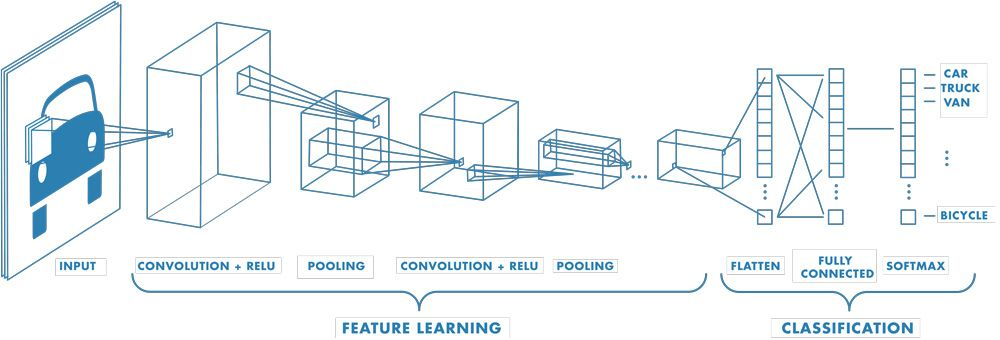
\includegraphics[width=0.95\columnwidth]{
                ../Imagens/CNN_mathworks.jpg
            }
            \caption{Arquitetura de uma rede convolucional. Filtros extratores de características são aplicados em diferentes resoluções e campos visuais. A saída de cada imagem convoluta alimenta a próxima camada. As ultimas camadas completamente conectadas realizam a classificação.}
            \label{fig:cnn}
        \end{figure}
    \end{frame}

\begin{frame}
\frametitle{Método}
    \begin{figure}[!ht]
        \centering
        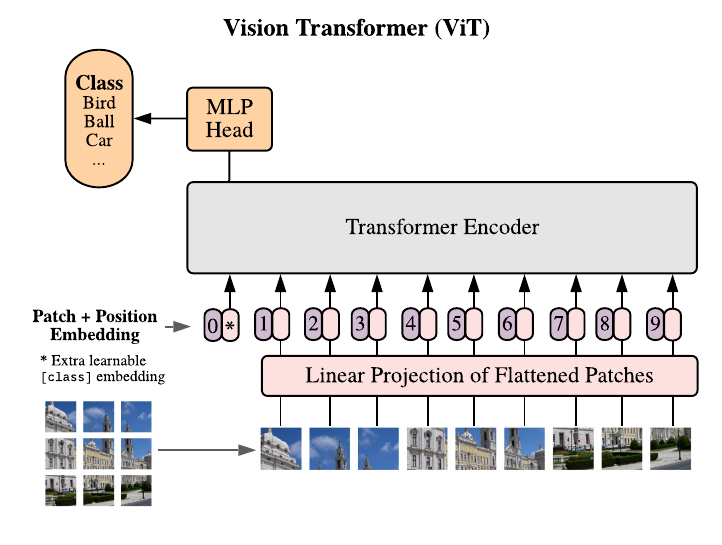
\includegraphics[width=0.5\columnwidth]{
            ../Imagens/vit.png
        }
        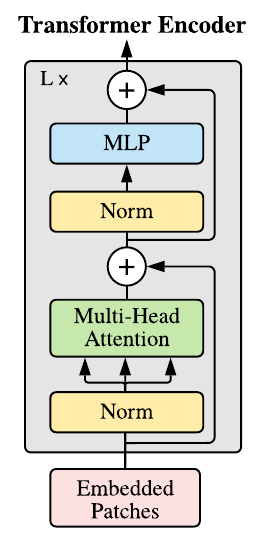
\includegraphics[width=0.2\columnwidth]{
            ../Imagens/encoder.png
        }
        \caption{O ViT divide uma imagem em uma grade de recortes quadrados, cada fragmento é achatado em um vetor único contendo todos canais de todos os pixeis, e projetando-os em uma dimensão de entrada desejada, alimentando a camada de múltiplos encoders em paralelo. \cite{dosovitskiy2020image}}
        \label{fig:vit}
\end{figure}
% Diante desse desafio, este trabalho consiste em utilizar técnicas estado da arte de visão computacional e aprendizado profundo para fazer classificações de regiões e capturas de satélites.

% Para isso serão testado modelos consolidados de visão, como o ResNet, bem como mais recentes, baseados em transformers visuais, o ViT. Também serão utilizadas técnicas de transferência de aprendizado, por meio de ajuste fino de modelo pré-treinados.
\end{frame}

\begin{frame}
\frametitle{Resultados e discussão}
\begin{figure}[!ht]
    \centering
    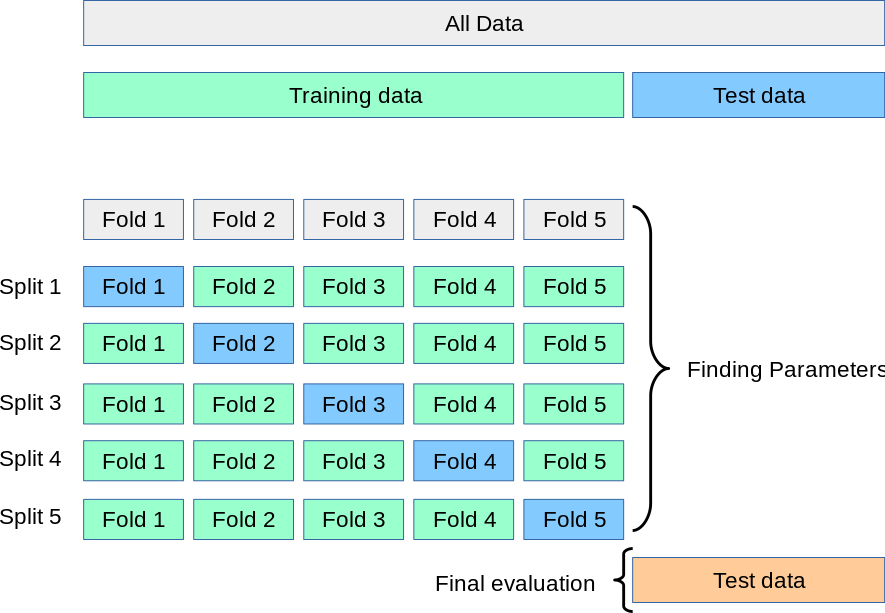
\includegraphics[width=0.45\columnwidth]{
        ../Imagens/validacao_cruzada.png
    }
    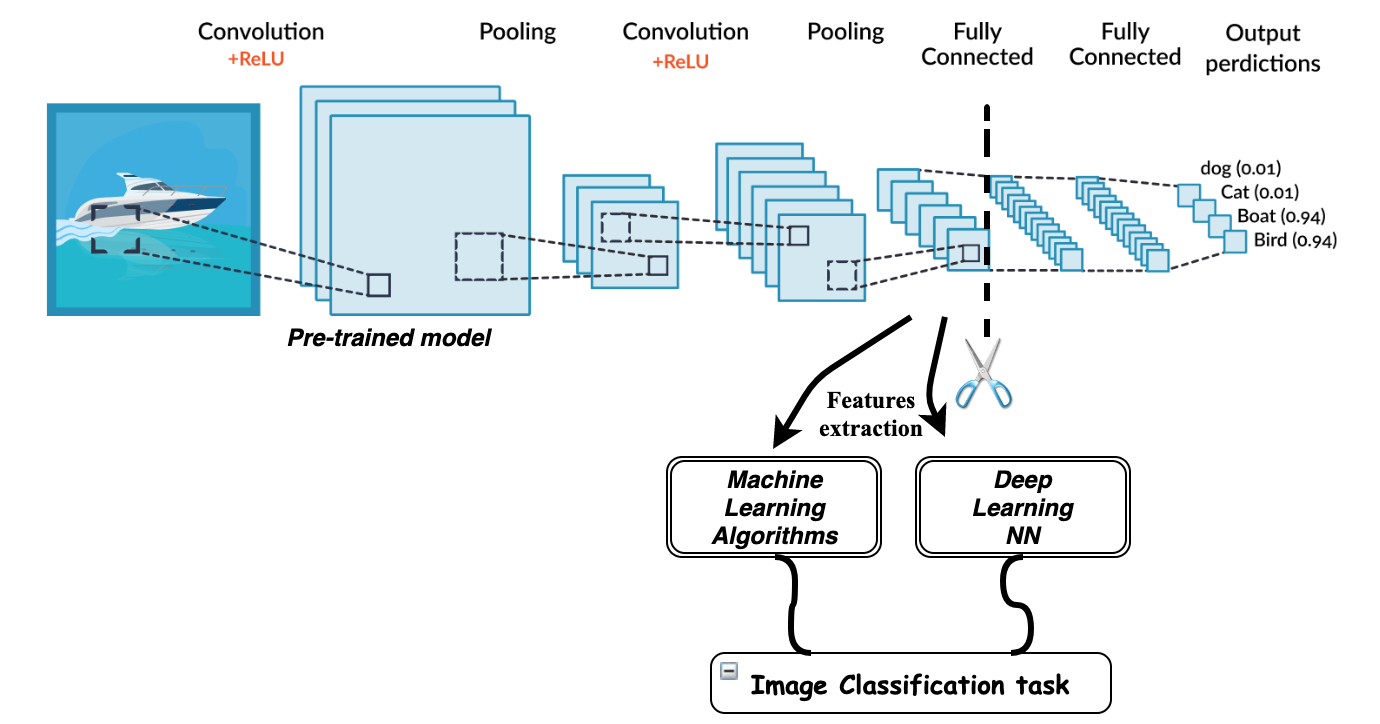
\includegraphics[width=0.45\columnwidth]{
        ../Imagens/fine_tune.png
    }
    \caption{O ViT divide uma imagem em uma grade de recortes quadrados, cada fragmento é achatado em um vetor único contendo todos canais de todos os pixeis, e projetando-os em uma dimensão de entrada desejada, alimentando a camada de múltiplos encoders em paralelo. \cite{dosovitskiy2020image}}
    \label{fig:vit}
\end{figure}
% Serão utilizados modelos pré-treinados em ../Imagens de sensoriamento remoto e serão experimentados se a partir do fine-tune generalizam bem o suficiente para serem utilizados na prática, nesta corrente aplicação. % Para avaliação dos resultados, também serão comparados com trabalhos bases. Serão aplicadas técinicas de validação como validação cruzada de 5 partições.

\end{frame}

\begin{frame}
\frametitle{Conclusão}
%Com o principal objetivo de aplicação de regiões irregulares como garimpo, agropecuária e desmatamento, este trabalho utilizará técnicas estado da arte de visão computacional e aprendizado profundo, bem como trabalhará arquiteturas como redes convolucionais e Transformers Visuais. 

\begin{figure}[!ht]
    \centering
    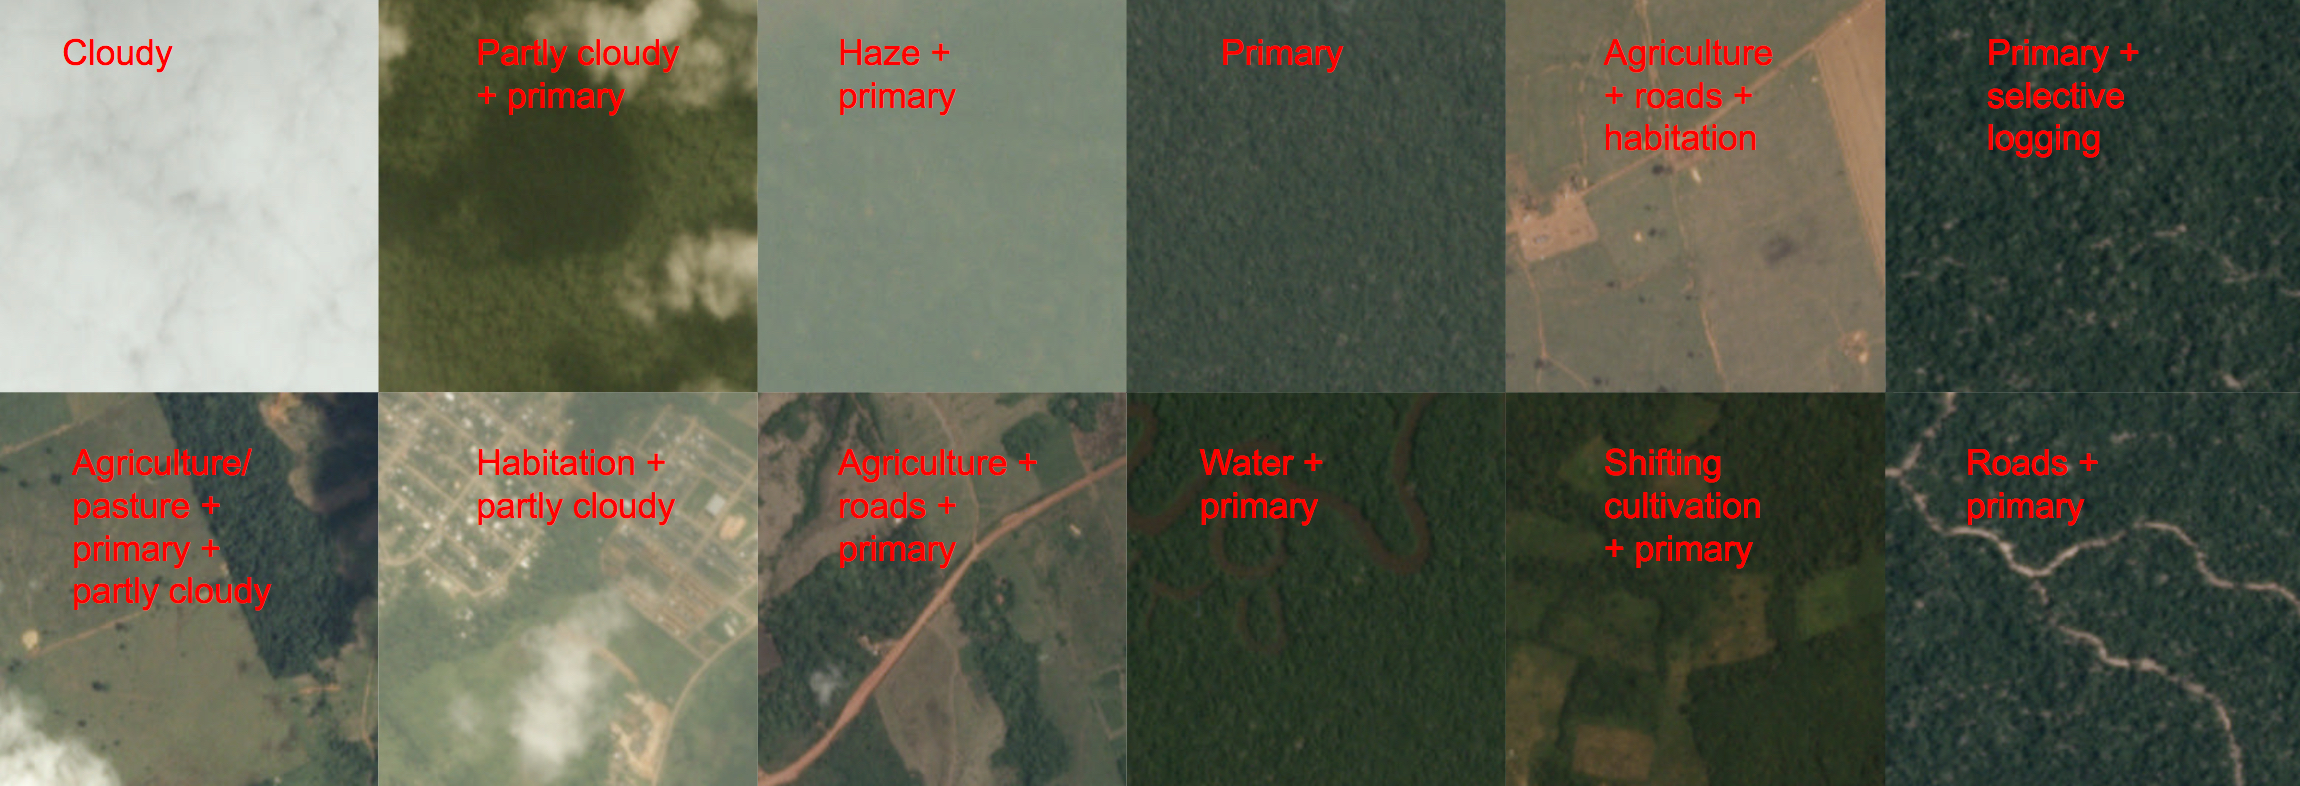
\includegraphics[width=0.9\columnwidth]{
        ../Imagens/chips.jpg
    }
    \caption{Amostras de classes do dataset Amazônia do espaço}\label{fig:dataset}
\end{figure}

\end{frame}



\end{document}








